\section{Project Scope}

From the literature survey and after talking with industry experts, the author found many issues that could be addressed when developing this system, but some of those problems like getting the models well optimized to react to anomalies is quickly is a very hard task to achieve. As this project is done by one developer in less than one year, it won't be possible to create a fully functional monitoring platform like Datadog or New Relic. So the focus of this project is to create an end-to-end framework that will make applying machine learning to solve \ac{sre} issues straightforward, so the future works can be built upon this project.

\subsection{In-scope} \label{sec:in-scope}
Following are the main focuses of this project
\begin{itemize}[noitemsep,nolistsep] 
    \item Low overhead data collection pipeline to collect service telemetry.
    \item Loosely coupled architectures, so all the components can be individually deployed.
    \item UI to easily visualize the service topology and identify root causes.
    \item Optimized models to have fairly small memory footprint and a CPU overhead.
    \item Well generalized model which will be able to deploy with completely new services and it will learn to adapt the new system.
    \item System should adopt to very large systems High Scalability.
    \item Interpretable models.
    \item Easily adaptable.
\end{itemize}


\subsection{Out-scope} \label{sec:out-scope}
Follow will not be covered during this project
\begin{itemize}[noitemsep,nolistsep]
    \item Working outside of Kubernetes eco-system.
    \item Intergrate with websockets.
    \item Acts as fully functional monitoring system.
    \item Multi-Cluster support
    \item Highly accurate predications from the model.
\end{itemize}

\subsection{Prototype Feature Diagram}
\begin{figure}[H]
    \centering
    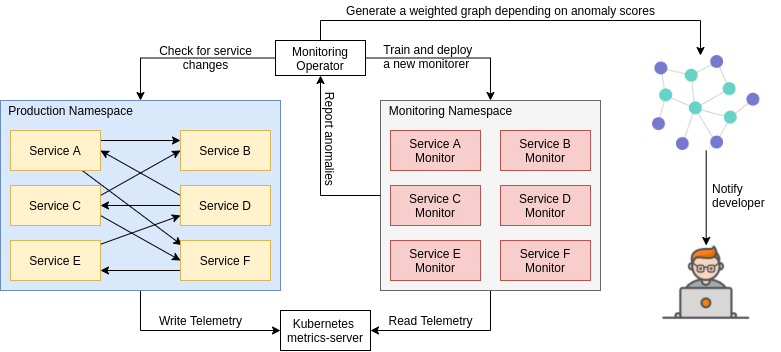
\includegraphics[width=16cm]{assets/introduction/High-level-system-diagram.png}
    \caption{Prototype feature diagram (self composed)}
    \label{fig:high-level-diagram}
\end{figure}